\documentclass[letterpaper,final,12pt,reqno]{amsart}

\usepackage[total={6.3in,9.2in},top=1.1in,left=1.1in]{geometry}

\usepackage{times,bm,bbm,empheq,fancyvrb,graphicx,amsthm,amssymb}
\usepackage[dvipsnames]{xcolor}
\usepackage{longtable}
\usepackage{booktabs}

\usepackage{tabto}
\TabPositions{1.5cm}

\usepackage{tikz}
\usetikzlibrary{decorations.pathreplacing}

\usepackage{float}

% hyperref should be the last package we load
\usepackage[pdftex,
colorlinks=true,
plainpages=false, % only if colorlinks=true
linkcolor=blue,   % ...
citecolor=Red,    % ...
urlcolor=black    % ...
]{hyperref}

\renewcommand{\baselinestretch}{1.05}

\allowdisplaybreaks[1]  % allow display breaks in align environments, if they avoid major underfulls

\newtheoremstyle{cstyle}% name
  {5pt}% space above
  {5pt}% space below
  {\itshape}% body font
  {}% indent amount
  {\itshape}% theorem head font
  {.}% punctuation after theorem head
  {.5em}% space after theorem head
  {\thmname{#1}\thmnumber{ #2}\thmnote{ (#3)}}% theorem head spec
\theoremstyle{cstyle}

\newtheorem{theorem}{Theorem}
\newtheorem{lemma}[theorem]{Lemma}
\newtheorem{assumptions}[theorem]{Assumptions}

\newtheoremstyle{cstyle*}% name
  {5pt}% space above
  {5pt}% space below
  {\itshape}% body font
  {}% indent amount
  {\itshape}% theorem head font
  {.}% punctuation after theorem head
  {.5em}% space after theorem head
  {\thmname{#1}}% theorem head spec
\theoremstyle{cstyle*}
\newtheorem{assumptions*}{Assumptions}

\newtheoremstyle{dstyle}% name
  {5pt}% space above
  {5pt}% space below
  {}%{\itshape}% body font
  {}% indent amount
  {\itshape}% theorem head font
  {.}% punctuation after theorem head
  {.5em}% space after theorem head
  {\thmname{#1}\thmnumber{ #2}\thmnote{ (#3)}}% theorem head spec
\theoremstyle{dstyle}

\newtheorem{definition}[theorem]{Definition}
\newtheorem{example}[theorem]{Example}

%% numbering
%\numberwithin{equation}{section}
%\numberwithin{figure}{section}
%\numberwithin{table}{section}
%\numberwithin{theorem}{section}

\newcommand{\eps}{\epsilon}

\newcommand{\RR}{\mathbb{R}}
\newcommand{\ZZ}{\mathbb{Z}}

\newcommand{\grad}{\nabla}
\newcommand{\Div}{\nabla\cdot}
\newcommand{\trace}{\operatorname{tr}}

\newcommand{\hbn}{\hat{\mathbf{n}}}

\newcommand{\bb}{\mathbf{b}}
\newcommand{\be}{\mathbf{e}}
\newcommand{\bbf}{\mathbf{f}}
\newcommand{\bg}{\mathbf{g}}
\newcommand{\bn}{\mathbf{n}}
\newcommand{\br}{\mathbf{r}}
\newcommand{\bu}{\mathbf{u}}
\newcommand{\bv}{\mathbf{v}}
\newcommand{\bw}{\mathbf{w}}
\newcommand{\bx}{\mathbf{x}}
\newcommand{\by}{\mathbf{y}}
\newcommand{\bz}{\mathbf{z}}

\newcommand{\bF}{\mathbf{F}}
\newcommand{\bV}{\mathbf{V}}
\newcommand{\bX}{\mathbf{X}}

\newcommand{\bxi}{\bm{\xi}}
\newcommand{\bzero}{\bm{0}}

\newcommand{\cK}{\mathcal{K}}
\newcommand{\cV}{\mathcal{V}}

\newcommand{\rhoi}{\rho_{\text{i}}}

\newcommand{\ip}[2]{\left<#1,#2\right>}

\newcommand{\maxR}{R^{\bm{\oplus}}}
\newcommand{\minR}{R^{\bm{\ominus}}}
\newcommand{\iR}{R^{\bullet}}

\newcommand{\nn}{{\text{n}}}
\newcommand{\pp}{{\text{p}}}
\newcommand{\qq}{{\text{q}}}
\newcommand{\rr}{{\text{r}}}

\newcommand{\supp}{\operatorname{supp}}
\newcommand{\Span}{\operatorname{span}}


\begin{document}
\title[A linear model for the coupled equations of glacier evolution]{A linear model for the coupled equations \\ of glacier evolution}

\author{Ed Bueler}

\date{\today}

\begin{abstract} FIXME
\end{abstract}

\maketitle

%\tableofcontents

\thispagestyle{empty}
%\bigskip

\newfloat{pseudofloat}{t}{xyz}[section]
\floatname{pseudofloat}{Algorithm}


\section{Introduction} \label{sec:intro}

The main problem of glaciology is to determine how the geometry of a glacier, especially the ice thickness and ice-covered area, change as determined by the climate experienced by the glacier, especially the surface mass balance.

This problem is interesting mathematically because the nontrivial equations for the bulk ice are coupled to the equation for surface changes.  Ignoring conservation of energy, as we do in these notes, the bulk ice equations are the system of conservation of mass and momentum.  Assuming incompressibility, the system is the Stokes equations for a very-viscous fluid \cite{Elmanetal2014,GreveBlatter2009}, which determine ice velocity and pressure from ice geometry and boundary stresses, but which involve no time derivatives.  On the other hand, surface changes are modeled by the surface kinematical equation, often called the kinematic boundary condition \cite{GreveBlatter2009}, which involve both the time derivative of the ice surface elevation and the surface value of the ice velocity.  The bulk ice and surface kinematics are nontrivially coupled because the ice geometry (e.g.~surface elevation) determines the domain on which the Stokes equations apply, while the surface kinematical equation includes the ice velocity as a source term in addition to the climatically-generated surface mass balance.

The full, coupled model is both an inequality-constrained free-boundary problem, because ice thickness is necessarily nonnegative, and also highly nonlinear because the viscosity of ice is strain-rate dependent (shear-thinning; see \cite{GreveBlatter2009}).  It then makes sense, especially when considering numerical solution methods, to construct a simpler linear model, one which nonetheless has the essential bulk-to-surface coupling.  These notes construct such a model.

In Section \ref{sec:model} we propose the continuum equations which combine a 3D elliptic partial differential equation (PDE), much simpler than the Stokes equations, with a surface equation analogous to the steady-state of a glacier.  This 2D surface equation is scalar, like the surface kinematical equation, and it has the coupling character of the glacier problem in the sense that the surface value of the 3D problem solution is involved.  However, in the linear model problem we can explicitly form the coupling term as a linear integral operator.  The analogy with the glacier problem is made clear in Section \ref{sec:analogy}, after which we consider numerical solutions in Section \ref{sec:numerical}, and then conclude.


\section{Model equations} \label{sec:model}

Our model problem is a 2D equation with both partial derivatives and integrals, namely equation \eqref{eq:modelproblem} below.  It is created from looking at a notional surface process on the top of a 3D domain.  We start with the 3D problem.

For length $\ell>0$ and height $h>0$ given, let $\Lambda = (0,\ell)^2\times (0,h)$ be the rectangular-solid in 3D, with coordinates $x,y,z$, $0<x,y<\ell$, and $0<z<h$.  We call the $z=0$ boundary the \emph{bottom} and the $z=h$ boundary the \emph{top}, and the remaining boundaries the \emph{sides}.  Let $g(x,y)$ be a given function on the top, defined for $0<x,y<\ell$.

Consider the following 3D Laplace equation problem, on $\Lambda$, for scalar solution $u(x,y,z)$:
\begin{subequations}
\label{eq:laplaceproblem}
\begin{align}
\grad^2 u &= 0 & &\text{in } \Lambda = (0,\ell)^2\times (0,h), \label{eq:laplaceproblemA} \\
u &= 0 & &\text{on the bottom and sides}, \label{eq:laplaceproblemB} \\
\frac{\partial u}{\partial z} &= g & &\text{on the top $z=h$}. \label{eq:laplaceproblemC}
\end{align}
\end{subequations}
Note that $\frac{\partial u}{\partial n}=\frac{\partial u}{\partial z}$ is the outward-normal derivative on top of $\Lambda$.  See Figure \ref{fig:laplaceproblem}.

\begin{figure}[ht]
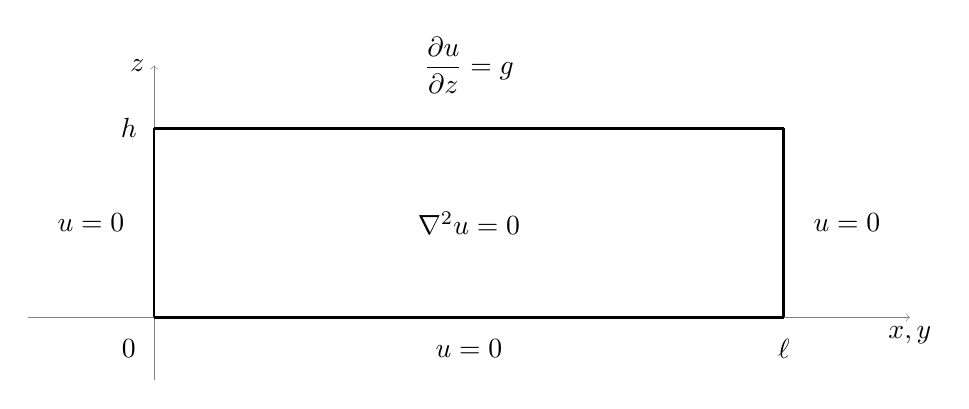
\begin{tikzpicture}[scale=8.0]
  % axes; x,y are horizontal and z is vertical
  \draw[->,gray,very thin] (-0.2,0.0) -- (1.2,0.0) node[below,black] {$x,y$};
  \draw[->,gray,very thin] (0.0,-0.1) -- (0.0,0.4) node[left,black] {$z$};
  % R = (0,L)^2
  \node at (-0.04,-0.05) {$0$};
  \node at (1.0,-0.05) {$\ell$};
  \node at (-0.04,0.3) {$h$};
  \draw[line width=1.0pt] (0.0,0.0) -- (0.0,0.3);
  \draw[line width=1.0pt] (1.0,0.0) -- (1.0,0.3);
  \draw[line width=1.0pt] (0.0,0.0) -- (1.0,0.0);
  \draw[line width=1.0pt] (0.0,0.3) -- (1.0,0.3);
  % equation and boundary conditions
  \node at (0.5,0.15) {$\grad^2 u = 0$};
  \node at (0.5,-0.05) {$u=0$};
  \node at (0.5,0.4) {$\displaystyle \frac{\partial u}{\partial z} = g$};
  \node at (-0.1,0.15) {$u=0$};
  \node at (1.1,0.15) {$u=0$};
\end{tikzpicture}
\caption{3D problem \eqref{eq:laplaceproblem} defines $u(x,y,z)$, for given Neumann condition $g(x,y)$.}
\label{fig:laplaceproblem}
\end{figure}

It is well-known that Laplace equation problem \eqref{eq:laplaceproblem} has a unique solution if $g$ is minimally well-behaved \cite{Elmanetal2014,Evans2010}.  The problem has a mixture of homogeneous Dirichlet (bottom and sides) and nonhomogeneous Neumann (top) boundary conditions; the fact that Dirichlet conditions apply on a positive-measure part of the boundary of $\Lambda$ implies uniqueness.

Thus it is reasonable to talk about \emph{the} solution $u$ of \eqref{eq:laplaceproblem} for given top-surface Neumann data $g$.  In particular we define a map from $g$ to the top-surface values, a trace \cite{Evans2010}, of the solution $u$.  Specifically, this is a linear \emph{Neumann-to-Dirichlet map},
\begin{equation}
N_h : \, g(x,y) \, \mapsto \, \frac{1}{h} u(x,y,h).  \label{eq:ntod}
\end{equation}
As shown in the Appendix, a separation of variables argument allows us to express this map as an integral against a known \emph{kernel} $K_h$, namely
\begin{equation}
(N_h g)(x,y) = \frac{1}{h} u(x,y,h) = \int_0^\ell \int_0^\ell K_h(x,y;\xi,\eta)\, g(\xi,\eta)\,d\xi\,d\eta  \label{eq:ntodformula}
\end{equation}
where
\begin{equation}
K_h(x,y;\xi,\eta) = (\text{FIXME: sum of $\sin() \sinh()$ products})  \label{eq:kernelformula}
\end{equation}

FIXME model problem is on 2D domain $\Omega = (0,\ell)^2$, with $\eps>0$:
\begin{equation}
-\eps \grad^2 s + N_h s = f  \label{eq:modelproblem}
\end{equation}
See Figure \ref{fig:modelproblem}.

\begin{figure}
\begin{tikzpicture}[scale=5.0]
  % axes
  \draw[->,gray,very thin] (-0.2,0.0) -- (1.2,0.0) node[below,black] {$x$};
  \draw[->,gray,very thin] (0.0,-0.2) -- (0.0,1.2) node[left,black] {$y$};
  % R = (0,L)^2
  \node at (-0.04,-0.05) {$0$};
  \node at (1.0,-0.05) {$\ell$};
  \node at (-0.04,1.0) {$\ell$};
  \draw[line width=1.0pt] (0.0,0.0) -- (0.0,1.0);
  \draw[line width=1.0pt] (1.0,0.0) -- (1.0,1.0);
  \draw[line width=1.0pt] (0.0,0.0) -- (1.0,0.0);
  \draw[line width=1.0pt] (0.0,1.0) -- (1.0,1.0);
  % equation and boundary conditions
  \node at (0.5,0.5) {$\displaystyle -\eps \grad^2 s + N_h s = f$};
  \node at (0.5,-0.1) {$s=0$};
  \node at (0.5,1.1) {$s=0$};
  \node[rotate=90] at (-0.1,0.5) {$s=0$};
  \node[rotate=-90] at (1.1,0.5) {$s=0$};
\end{tikzpicture}
\caption{Model problem \eqref{eq:modelproblem} on $\Omega = (0,\ell)^2$.}
\label{fig:modelproblem}
\end{figure}

FIXME alternative model has ``$N_h \grad s$'' instead of $N_h s$, in some form?

FIXME observe how $N_h s$ behaves as $h\to 0$

FIXME much more to write


\section{Analogy with the steady and implicit-step glacier problems} \label{sec:analogy}

FIXME


\section{On multigrid solutions of \eqref{eq:modelproblem}} \label{sec:numerical}

FIXME \cite{Briggsetal2000,Bueler2021,Trottenbergetal2001} for multigrid

FIXME need to explore smoothers which can handle the $N_h$ integral operator

\section{Discussion and Conclusion} \label{sec:conclusion}

FIXME \cite{Girouardetal2022} show that the Neumann-to-Dirichlet map $\mathcal{N}:\frac{\partial u}{\partial n}|_{\partial} \mapsto u|_{\partial}$ along the \emph{entire} boundary of a 3D domain $\Lambda \subset \RR^3$ is very close to $|\grad_{\partial}|^{-1}$ where $|\grad_{\partial}| = \sqrt{-\grad_{\partial}^2}$ is the square root of the positive boundary Laplacian $-\grad_{\partial}^2$; they are identical only when $\Omega$ is a 3D sphere, which is not true here

\bibliography{model}
\bibliographystyle{siam}


\appendix
\section{Laplace problem Neumann-to-Dirichlet operator}

In this section we give an explicit formula for the solution of the 3D Laplace equation problem \eqref{eq:laplaceproblem}, the problem illustrated in Figure \ref{fig:laplaceproblem}.  The explicit formula is an infinite series coming from a classical separation-of-variables type solution.  (A closed, non-series form may exist but it is not known to the authors.)  The goal is to derive kernel formula \eqref{eq:kernelformula}, the kernel of the Neumann-to-Dirichlet operator $N_h$, in a verifiable manner.

Consider the orthogonal set
    $$\left\{\,\sin(j\pi x/\ell)\,\right\}$$
for $j=1,2,\dots$, i.e.~$j\in \ZZ$, which is a basis of $L^2(0,\ell)$.  Recall the following formulas:
\begin{align*}
&\int_0^\ell \sin(j\pi x/\ell) \sin(k\pi x/\ell)\,dx = \begin{cases} 0, & j \ne k \\ \ell/2, & j=k \end{cases} \\
&f(x) = \sum_{j=1}^\infty c_j \sin(j\pi x/\ell) \qquad \iff \qquad c_j = \frac{2}{\ell} \int_0^\ell f(x) \sin(j\pi x/\ell)\,dx
\end{align*}

It follows that, on the 2D domain $\Omega = (0,\ell)^2$, if $g\in L^2(\Omega)$ then
    $$g(x,y) = \sum_{j=1}^\infty \sum_{k=1}^\infty c_{jk} \sin(j\pi x/\ell) \sin(k\pi y/\ell)$$
where
    $$c_{jk} = \frac{4}{\ell^2} \int_0^\ell \int_0^\ell g(x,y) \sin(j\pi x/\ell) \sin(k\pi y/\ell)\,dx\,dy.$$

On the other hand, it is easily checked that for each index pair $j,k \in \ZZ$, the following function solves equations \eqref{eq:laplaceproblemA} and \eqref{eq:laplaceproblemB}, that is, it solves the homogeneous parts of the 3D Laplace equation problem:
    $$v_{jk}(x,y,z) = \sin(j\pi x/\ell) \sin(k\pi y/\ell) \sinh(\sqrt{j^2+k^2}\, \pi z/\ell).$$
By linearity this infinite sum also solves equations \eqref{eq:laplaceproblemA} and \eqref{eq:laplaceproblemB}:
    $$u(x,y,z) = \sum_{j=1}^\infty \sum_{k=1}^\infty a_{jk} v_{jk}(x,y,z)$$

We seek to satisfy condition \eqref{eq:laplaceproblemC} for a given $g(x,y)$.  Note
    $$\frac{\partial u}{\partial z}(x,y,h) = \sum_{j=1}^\infty \sum_{k=1}^\infty \frac{\sqrt{j^2+k^2}\, \pi}{\ell} a_{jk} \sin(j\pi x/\ell) \sin(k\pi y/\ell) \cosh(\sqrt{j^2+k^2}\, \pi h/\ell)$$
It follows from uniqueness of coefficients, i.e.~orthogonality, that
    $$g(x,y) = \frac{\partial u}{\partial z}(x,y,h) \qquad \iff \qquad a_{jk} = \frac{\ell}{\sqrt{j^2+k^2} \cosh(\sqrt{j^2+k^2}\, \pi h/\ell)} \,c_{jk}$$
where $c_{jk}$ are computed from $g(x,y)$ by the integral formula above.  Recalling that
    $$(N_h g)(x,y) = \frac{1}{h} u(x,y,h),$$
we have the following integral formula for $N_h g$,
    $$(N_h g)(x,y) = \int_0^\ell \int_0^\ell K_h(x,y;\xi,\eta)\, g(\xi,\eta)\,d\xi\,d\eta$$
where
    $$K_h = \text{FIXME plug and plug}.$$
This justifies \eqref{eq:kernelformula}.
\end{document}
